\documentclass{article}
\usepackage[utf8]{inputenc}
\usepackage{amsmath}
\usepackage{graphicx}
\usepackage{hyperref}
\usepackage{tikz}
\usepackage[a4paper,margin=1in,footskip=0.25in]{geometry}

\title{\textbf{Hypothetical Interventions on Sleep Stage Composition and Cognition and Brain Health} \protect\\ Analysis Plan}
\author{Lachlan Cribb, Beaudan Brown, Stephanie Yiallourou, Matthew Pas\'e}
\date{\today}
\setlength{\parskip}{0.75em}
\begin{document}

\maketitle

\section{Introduction}
In epidemiology, compositional exposures are multivariate exposures constrained to a constant sum. For example, the time spent in sleep, inactivity, and physical activity are compositional components of a 24-hour day. This constraint poses problems for studies aiming to estimate the effect of intervening on such exposures. For one, the perfect collinearity among the composition elements makes traditional statistical methods, like multivariable regression, unsuitable. While this issue is often avoided in practice by focusing on one element of the composition at a time (i.e., without holding the other components constant), the question addressed using this approach is then ill-defined: it represents the effect of increasing one component while reducing the other components by an equivalent amount in an unspecified way. For example, increasing total physical activity time at the expense of reduced time in some unspecified combination of inactivity and sleep.

Another compositional exposure that is of growing interest in the dementia setting is the proportion of total sleep time spent in different sleep stages. Insufficient slow wave sleep (SWS) has been associated with increased risk of dementia \cite{himali_association_2023}. SWS is thought to be important for glymphatic clearance of amyloid-$\beta$ and tau, the two hallmark features of Alzheimer's disease dementia. Restoring SWS may therefore reflect a potential intervention target to reduce risk of dementia. Similarly, an excessive proportion of time spent in light sleep (N1) has been associated with cognitive decline in older people \cite{song_relationships_2015}. A difficulty in interpreting these results, however, is the compositional nature of sleep stages within a fixed sleep window. An increase in SWS, for example, must come at the expense of some combination of N1, N2, REM, and WASO, or otherwise from an increased overall sleep duration (i.e., at the expense of wake). It may well be that the effect of increasing time in SWS depends on which state(s) that time comes at the expense of.

We can overcome the issues of perfect multicollinearity and ill-defined interventions using the compositional data analysis (CoDA) approach. This approach involves first mapping the original $J$ dimensional composition into a $J-1$ dimensional set of log-ratio coordinates \cite{aitchisonStatisticalAnalysisCompositional1982}. The interventions of interest are then defined as explicit \textit{substitutions} applied to the composition. For example, increasing time in SWS by 5 minutes and reducing time in WASO by 5 minutes. Finally, the effect of these substitutions can be estimated using g-computation, inverse-probability weighting, or their doubly-robust extensions. These statistical approaches have advantages over conventional outcome regression-based approaches, including 1. they do not require interpretation of the regression coefficients for log-ratio coordinates, which, especially when the form of the outcome regression is complex and/or the composition is high-dimensional, is difficult; and 2. they generalise to longitudinal treatments with time-varying confounding.


\section{Aims}
\begin{enumerate}
    \item To investigate the effect of different hypothetical interventions on sleep stage composition (the proportion of time spent in each state within a fixed sleep window; N1, N2, N3/N4, REM, and WASO) on the risk of cognitive decline and MRI volumetric outcomes, compared to no intervention (not changing the sleep stage composition).
    \item To find the "lowest risk" and "highest risk" pattern of sleep stage compositions with respect to risk of cognitive impairment. I.e., the absolute quantities of time spent in each state which is associated with the highest/lowest risk of cognitive decline.
\end{enumerate}

\section{Methods}

\subsection{Observational data}

Data are obtained from the Framingham Offspring Study (FOS) and the Sleep Heart Health Study (SHHS). SHHS is a multi-centre prospective cohort study designed to examine the cardiovascular outcomes of sleep-disordered breathing in middle-aged and older adults. Participants were recruited from multiple parent cohorts, including FOS, the Atherosclerosis Risk in Communities (ARIC) cohort, and the Cardiovascular Health Study (CHS). For this study, we used SHHS data provided by participants from the FOS study.

For SHHS, a sample of participants who met the inclusion criteria (see below) was invited to participate in the baseline SHHS examination (SHHS-1), which included a polysomnogram. A total of 997 individuals from the FOS study were enrolled between 1995 and 1998. A second polysomnogram (SHHS-2) was performed between 2001 and 2003 in 638 FOS participants.

\subsubsection{Eligibility criteria}

The following are the eligibility criteria for participation in SHHS:

\begin{itemize}
    \item Aged 40 or older
    \item No history of treatment for sleep apnea
    \item no Tracheostomy
    \item No current home oxygen therapy
\end{itemize}

\noindent For this study, we will additionally require that participants have SHHS-1 and SHHS-2 polysomnography data available and apply the following exclusion criteria:

\begin{itemize}
    \item Dementia or other significant neurological disease prior to SHHS-2
    \item Mild cognitive impairment prior to SHHS-2
    \item Significant cardiovascular disease prior to SHHS-2
    \item Less than 4 hours of sleep at SHHS-1 or SHHS-2
\end{itemize}

\subsection{Hypothetical interventions}

Our exposure of interest is the sleep stage composition at SHHS-2, represented by $A = (A_1, A_2, A_3, A_4, A_5) = (N1, N2, N3/N4, REM, WASO)$, where $A_j$ denotes time spent in sleep stage $j \in \{1,...,5\}$. We use SHHS-2, rather than SHHS-1, for our exposure variables because it allows us to statistically adjust for sleep stage composition at SHHS-1. This ensures that the SHHS-2 sleep composition is approximately an "incident" exposure, reducing confounding and selection bias related to past sleep behaviours.

The reference composition is the observed sleep stage composition $A$. We consider hypothetical isotemporal substitution interventions that redistribute time between two sleep stages while holding the total sleep window fixed. We denote these compositional interventions by $d$ and the composition resulting from this intervention as $d(A)$. For example, the intervention $d(A) = A + \Delta$, where $\Delta = (0, 0, 5, -5, 0)$ increases time in SWS $A_3$ and reduces time in REM $A_4$ by 5 minutes. A potential issue with this intervention $d$, however, is that $d(A)$ may not lie within the support of the data. For someone with only 3 minutes of REM, for example, an intervention to reduce REM by 5 minutes would result in -2 minutes of REM, which is obviously impossible. More generally, interventions $d$ that produce compositions that are not within the support of the data will rely purely on extrapolation, which is unlikely to be valid.

Accordingly, following \cite{rudolphEverythingAllOnce2025}, we utilise the convex hull to ensure that the compositional interventions stay within the support of the data. In our case, the convex hull is the smallest $J-1 = 4$ dimensional polygon (a subspace of the 4-simplex) that contains all of the observed exposure values. Any data outside of the borders of the convex hull will require extrapolation. We will compute the convex hull for our exposure data using the Julia software. Note, however, that we are only able to compute the convex hull the \textit{marginal} distribution of the exposures, rather than the distribution of the exposures conditional on the covariates. Though the latter is what is important for avoiding extrapolation and for the positivity assumption (see below) to hold, the former is a useful approximation \cite{rudolphEverythingAllOnce2025}.

We now define the intervention $d$, incorporating the data support constraint:

\[
    d(A) =
    \begin{cases}
        A + \Delta & \text{if} A + \Delta \in \text{convex hull}, \\
        A          & \text{otherwise}
    \end{cases}
\]

Where $\Delta$ is a vector of length $J$ with $\sum_{j=1}^{J} \Delta_j = 0$.

\subsection{Outcomes}
\begin{itemize}
    \item Time to cognitive impairment, a composite of cognitive decline or dementia
    \item MRI volumetric outcomes (total brain volume, grey matter volume, white matter volume, hippocampal volume, white matter hyperintensities)
\end{itemize}

\subsection{Follow-up}
Follow-up commences at the time of SHHS-2 (the time of exposure measurement). Follow-up ends at loss to follow-up, death, or outcome measurement.

\subsection{Causal contrast}

For survival outcomes, our causal contrast of interest is the total effect \cite{youngCausalFrameworkClassical2020b} of the intervention $d$ on the risk of cognitive impairment $E[Y^{A^d} - Y]$. This represents the effect of the intervention through all pathways, including through the competing event of death. For the MRI outcomes, as MRI outcomes are undefined after death occurs, our estimand is the average causal effect in survivors $E[Y^{A^d} - Y|D=0]$, where $D$ = death. Implicit in each causal contrast is an intervention to abolish censoring throughout follow-up.


\subsection{Confounders}

The presumed structure of confounding is displayed in the directed acyclic graph in Figure \ref{fig:dag}. $A$ represents sleep stage composition at SHHS-2, which is the exposure. $L_0$ represents confounders measured before but proximal to SHHS-2 and includes age, sex, education, race, MMSE score, body mass index (BMI), waist circumference, physical activity (from the PAI), hypertension, CVD, diabetes, smoking status, APOE $\epsilon$ 4 positivity, medication (sedative, sleeping pill, antidepressant), apnea hypopnea index, MRI intracranial volume (for MRI outcomes only), SHHS1 Sleep macro-architecture measures (i.e., time in N1, N2, N3, REM, time awake, wake after sleep onset) mapped to log ratio coordinates, and SHHS1 sleep maintenance efficiency and apnea hypopnea index. $L$ represents covariates variables measured at time $t$ which are common causes of censoring and the outcome. $U$ is a vector of unmeasured variables (e.g., genetics) which is a common cause of sleep stage composition, covariates $L_t$, death $D$, and the outcome $Y$.

\begin{figure}[h]
    \centering
    \usetikzlibrary{positioning}
    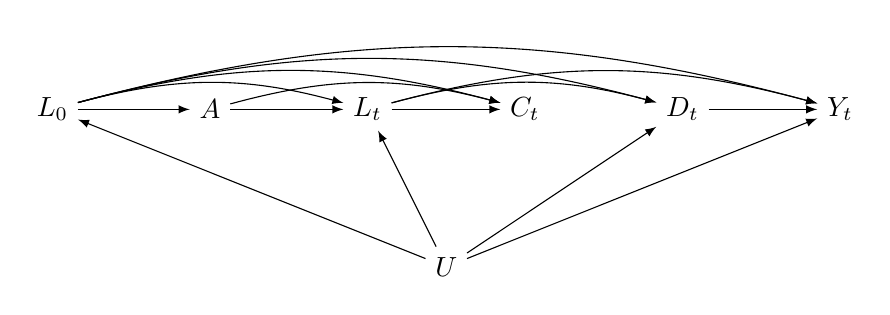
\begin{tikzpicture}[every node/.append style={draw, minimum size=0.5cm}]
        \node [draw=none] (L0) at (0,0) {$L_{0}$};
        \node [draw=none] (A) at (2,0) {$A$};
        \node [draw=none] (L) at (4,0) {$L_t$};
        \node [draw=none] (C) at (6,0) {$C_t$};
        \node [draw=none] (D) at (8,0) {$D_t$};
        \node [draw=none] (Y) at (10,0) {$Y_t$};
        \node [draw=none] (U) at (5,-2) {$U$};

        \draw [-latex] (L0) edge (A);
        \draw [-latex] (L0) edge [bend left=15] (L);
        \draw [-latex] (L0) edge [bend left=15](D);
        \draw [-latex] (L0) edge [bend left=15] (Y);
        \draw [-latex] (L0) edge [bend left=15] (C);
        \draw [-latex] (L) edge [bend left=15] (D);
        \draw [-latex] (L) edge [bend left=15] (Y);
        \draw [-latex] (L) edge (C);
        \draw [-latex] (A) edge (L);
        \draw [-latex] (A) edge [bend left=15] (C);
        \draw [-latex] (U) edge (D);
        \draw [-latex] (U) edge (Y);
        \draw [-latex] (U) edge (L0);
        \draw [-latex] (U) edge (L);
        \draw [-latex] (D) edge (Y);
    \end{tikzpicture}
    \caption{Directed acyclic graph}
    \label{fig:dag}
\end{figure}

Note that, for the MRI outcomes, the identification of the average causal effect in survivors requires that the exposure $A$ is independent of $D$.

\subsection{Statistical analysis}

\subsubsection{Isotemporal substitutions}

For the primary analysis, we will use g-computation to estimate the substitution effects. For the time to cognitive impairment outcome, the steps for this algorithm are:
\begin{enumerate}
    \item Apply the intervention to create $A^d$
    \item Map $A$ and $A^d$ from the simplex to the Real space using an isometric log ratio (ILR) transformation
    \item Fit a pooled over time logistic model for $Y$ and for $D$, given $ILR(A)$ and the baseline confounders. This model will include restricted cubic splines (knots at the 5th, 50th, and 95th percentiles) for continuous variables and two-way product terms between the exposures and time, key confounders (age, sex, APOE, education) and time, and between the key confounders.
    \item Generate predicted hazards for $Y$ and $D$ with the exposures set $ILR(A)$ (reference) and $ILR(A^d)$ (intervention)
    \item For each intervention, compute risks as a function of the estimated hazards. Then, average the estimated risks over the baseline covariates $L_0$.
    \item Calculate the effect estimate as the difference between interventions
    \item Perform 500 replications of the non-parametric bootstrap for percentile based 95\% confidence intervals
\end{enumerate}

The specification of the outcome model for the MRI outcomes will be equivalent, though no time term will be required.


\subsubsection{Highest and lowest risk compositions}

To estimate the highest and lowest composition, i.e., the absolute time spent in each sleep stage associated with the best and worst outcome, respectively, we will use the following method:
\begin{enumerate}
    \item
\end{enumerate}

\subsection{Sensitivity analyses}


\section{References}
\bibliographystyle{plain}
\bibliography{citations}

\end{document}
